\documentclass[fleqn]{article}
\oddsidemargin 0.0in
\textwidth 6.0in
\thispagestyle{empty}
\usepackage{import}
\usepackage{amsmath}
\usepackage{amssymb}
\usepackage{graphicx}
\usepackage[english]{babel}
\usepackage[utf8x]{inputenc}
\usepackage{float}
\usepackage{bigints} 
\usepackage[colorinlistoftodos]{todonotes}
\usepackage{setspace}
\usepackage{geometry}
\usepackage{colortbl}
\usepackage{xcolor,colortbl}

\newcommand{\va}{\mbox{\boldmath{$a$}}}
\newcommand{\vb}{\mbox{\boldmath{$b$}}}
\newcommand{\vc}{\mbox{\boldmath{$c$}}}
\newcommand{\vd}{\mbox{\boldmath{$d$}}}
\newcommand{\vi}{\mbox{\boldmath{$i$}}}
\newcommand{\vj}{\mbox{\boldmath{$j$}}}
\newcommand{\vk}{\mbox{\boldmath{$k$}}}
\newcommand{\vr}{\mbox{\boldmath{$r$}}}
\newcommand{\vectr}[1]{\mbox{\boldmath{${#1}$}}}
\newcommand{\unitvec}[1]{\mbox{\boldmath{$\hat{#1}$}}}
\newcommand{\matA}{\mbox{$\underline{\underline{A}}$}}
\newcommand{\matB}{\mbox{$\underline{\underline{B}}$}}
\newcommand{\matAtranspose}{\mbox{$\underline{\underline{\tilde{A}}}$}}
\newcommand{\matBtranspose}{\mbox{$\underline{\underline{\tilde{B}}}$}}
\newcommand{\matone}{$\underline{\underline{I}}$}
\newcommand{\grad}[1]{\mbox{\boldmath $\nabla$}\mbox{$#1$}}
\newcommand{\divg}[1]{\mbox{\boldmath $\nabla$} \mbox{$\cdot$} \mbox{\boldmath $#1$}}
\newcommand{\curl}[1]{\mbox{\boldmath $\nabla$} \mbox{$\times$} \mbox{\boldmath $#1$}}

\definecolor{hwColor}{HTML}{AD53BA}
\definecolor{contents}{HTML}{EAFF7C}
\definecolor{red}{HTML}{FF0000}

\doublespacing
\begin{document}

\begin{titlepage}

\newcommand{\HRule}{\rule{\linewidth}{0.5mm}} % Defines a new command for the horizontal lines, change thickness here

\center % Center everything on the page
 

\textsc{\LARGE Arizona State University}\\[1.5cm] 

\textsc{\LARGE Mathematical Methods For Physics II }\\[1.5cm]


\begin{figure}
  
\includegraphics[width=\linewidth]{asu.png}
\end{figure}


\HRule \\[0.4cm]
{ \huge \bfseries Portfolio}\\[0.4cm] 
\HRule \\[1.5cm]
 
\textbf{Behnam Amiri}

\bigbreak

\textbf{Prof: Cecilia Lunardini (Grader. Kenna McRae)}

\bigbreak


\textbf{{\large \today}\\[2cm]}

\vfill

\end{titlepage}

\huge \textbf{Academic integrity statement:}

\bigbreak

\Large I am aware of the course rules detailed in the syllabus and related course documents. I am also aware of Arizona State University’s policies and practices against plagiarism and other forms of academic dishonesty. I affirm that I have not given or received any unauthorized help on this assignment, and I have not used any unauthorized resources. All authorized help (from the instructor, or learning assistant), authorized collaborations (with classmates), and authorized resources are explicitly stated and described in detail in the present document.

\bigbreak

\Large This work is entirely my own, except when collaboration with classmates is explicitly declared, and I take full responsibility for it.

\bigbreak

\Large Signature and date:

\bigbreak

\bigbreak


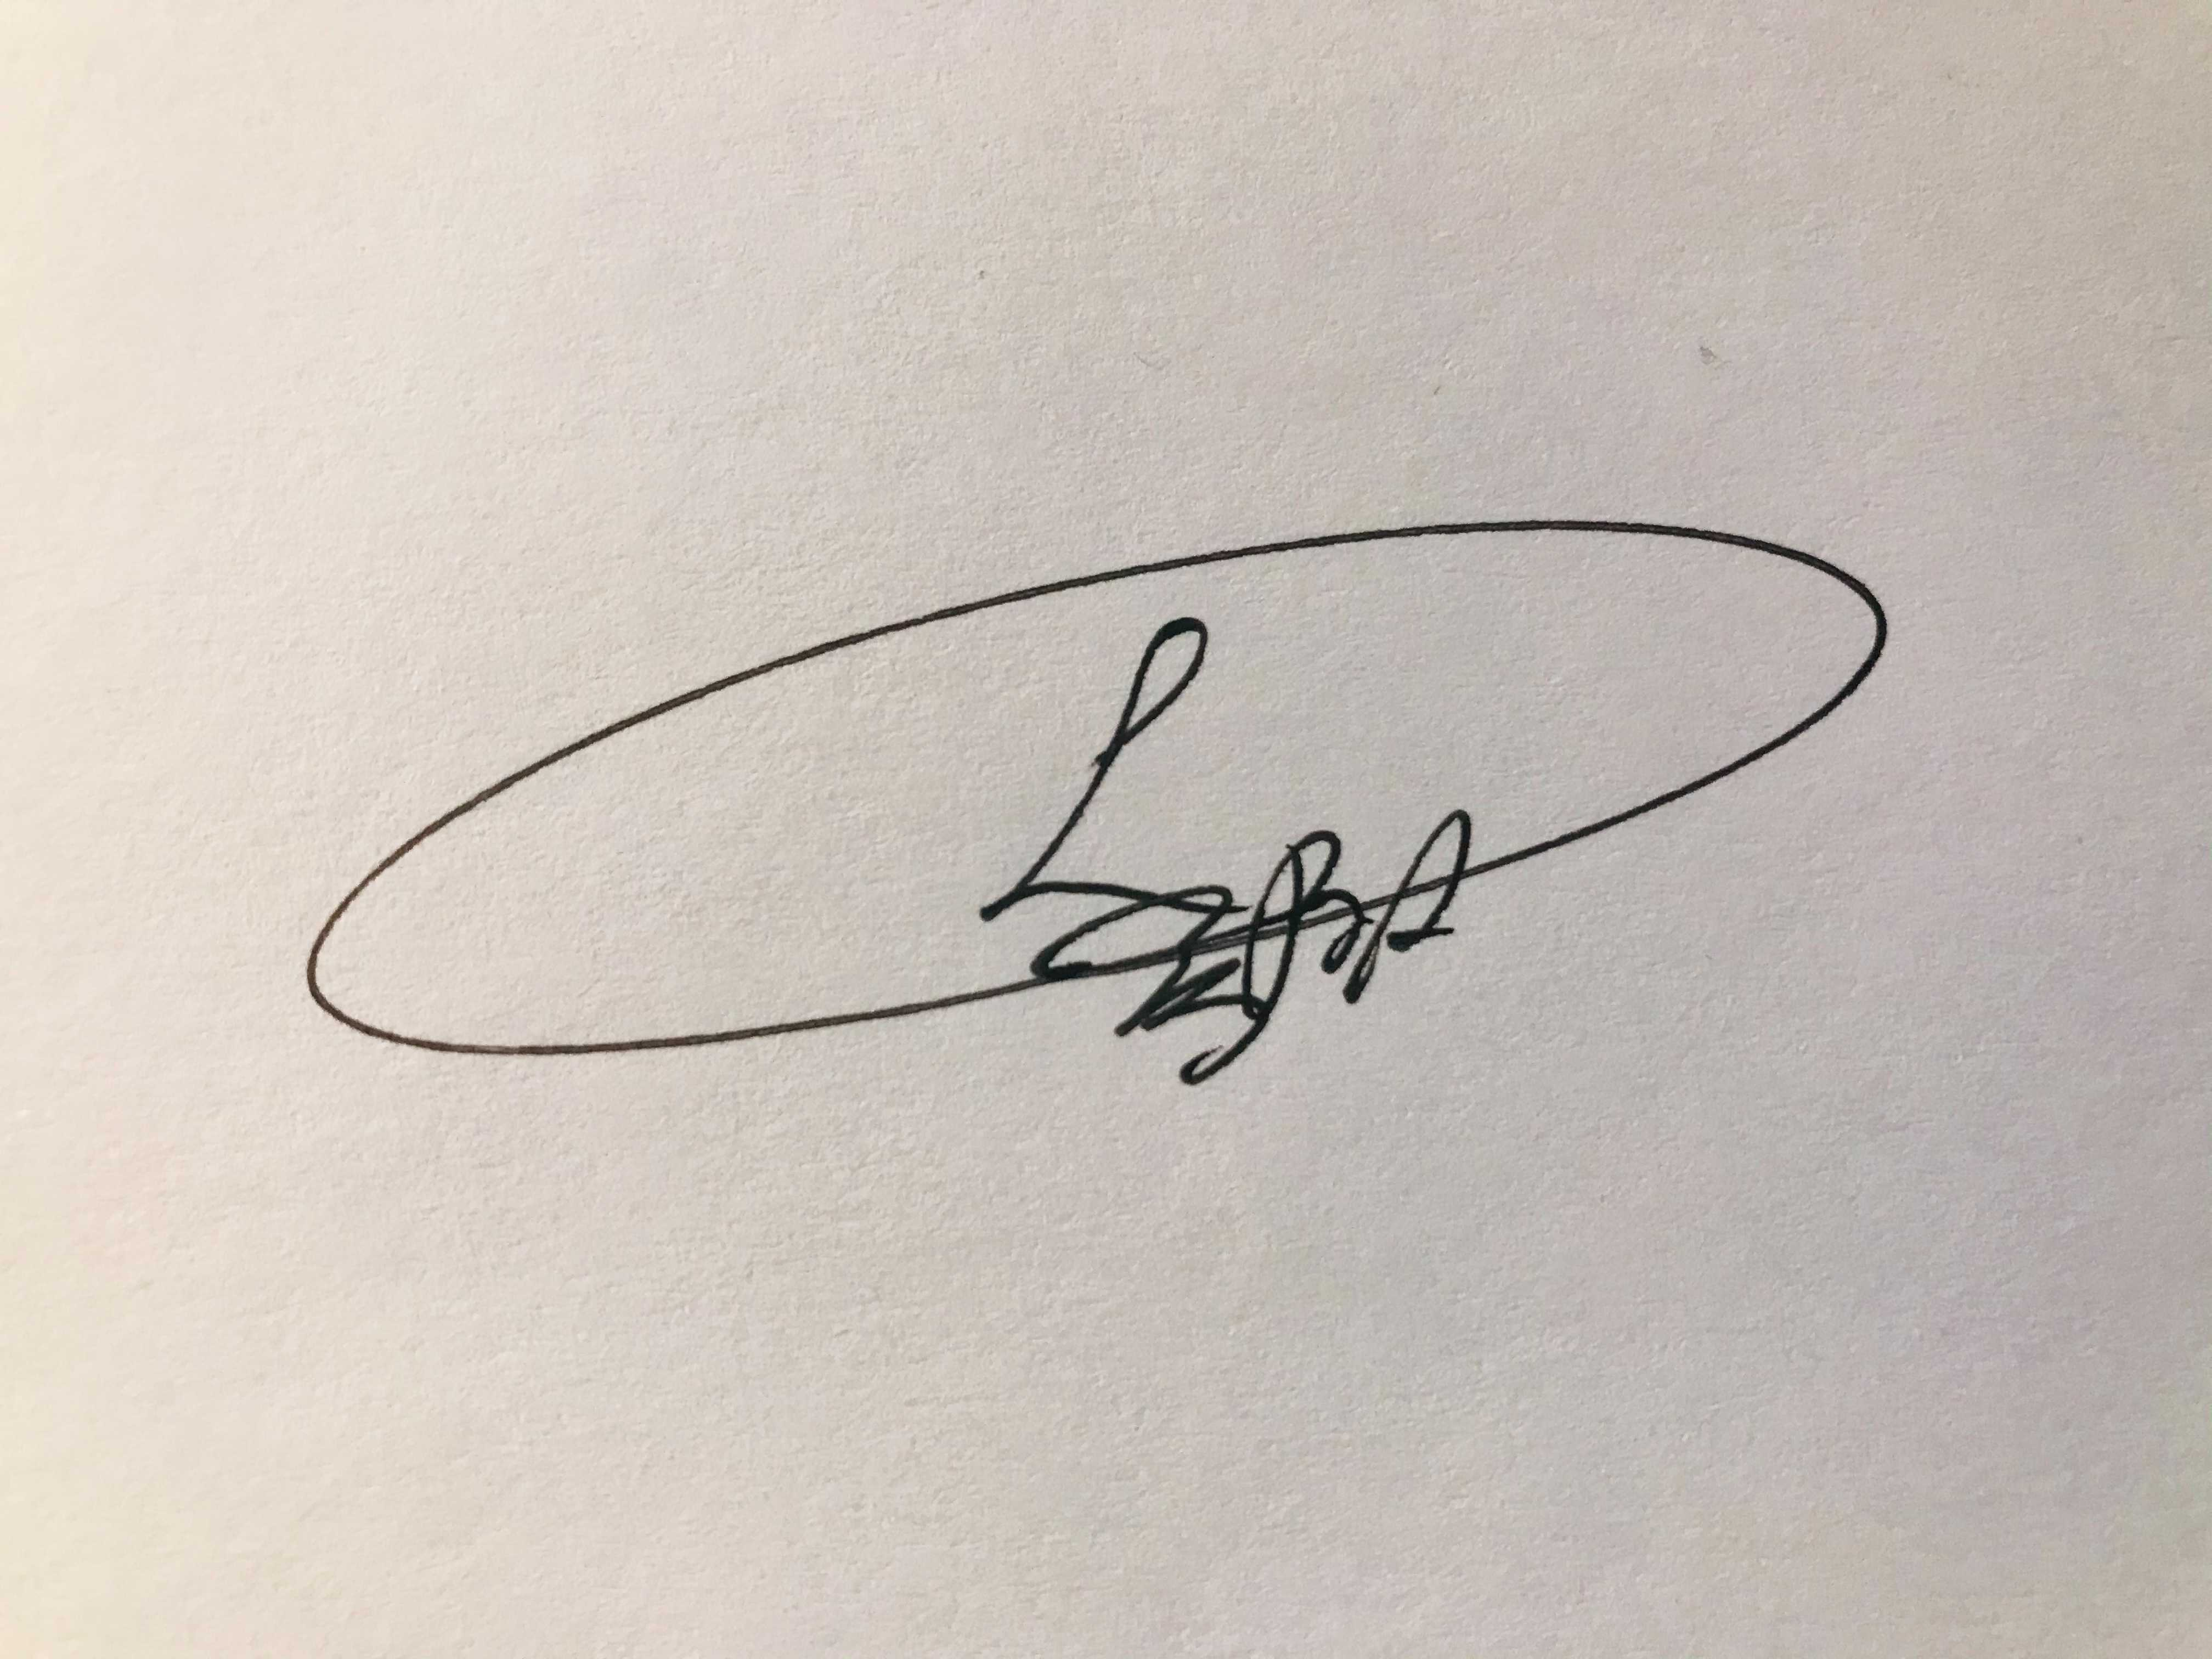
\includegraphics[height=3cm, width=6cm]{signature.jpg}

\Large \textbf{ Behnam Amiri, \today }


\pagebreak

%  Table of contents
\begin{singlespace}
  \begin{tabular}{ |p{3cm}|||p{4cm}|p{2cm}|p{2cm}|p{2cm}|  }
      \hline
      Topic & Assignment & Page & Point Value & Points Earned \\
      \hline
      Vector Calculus & \cellcolor{contents} Problems/Other & \cellcolor{contents} 3 &\cellcolor{contents}  ... &\cellcolor{contents}  ... \\
      & \cellcolor{contents} Exercises &\cellcolor{contents}  6 & \cellcolor{contents}  ... &\cellcolor{contents}  ... \\
      \hline
      Line, surface and volume integrals & Problems/Other & ... & ... & ... \\
      & Exercises & ... & ... & ... \\
      \hline
      Integral transforms & \cellcolor{contents} Problems/Other &\cellcolor{contents}  ... &\cellcolor{contents}  ... & \cellcolor{contents} ... \\
      & \cellcolor{contents} Exercises &\cellcolor{contents}  ... &\cellcolor{contents}  ... &\cellcolor{contents}  ... \\
      \hline
      Special functions & Problems/Other & ... & ... & ... \\
      & Exercises & ... & ... & ... \\
      \hline
      Partial differential equations  &\cellcolor{contents} Problems/Other &\cellcolor{contents} ... &\cellcolor{contents} ... &\cellcolor{contents} ... \\
      & \cellcolor{contents} Exercises &\cellcolor{contents}  ... &\cellcolor{contents}  ... &\cellcolor{contents}  ... \\
      \hline
      Complex functions of a complex variable & Problems/Other & ...  & ... & ... \\
      & Exercises  & ...  & ... & ... \\
      \hline
      Total & ... & ... & ... & ... \\
      \hline
  \end{tabular}
\end{singlespace}

\pagebreak

\vfill

  \emph{ Important reminder: to get full credit, all calculations must be done by hand, without using electronic devices. Steps must be reasonably detailed.  The use of electronic devices is allowed, but must be explicitly declared, and will result in partial credit. See syllabus for details. Also see syllabus for rules on collaborating with others on a problem. } 

  \pagebreak 

  \textbf{Problem sets on Vector calculus} (40 points)
  \begin{enumerate}

    \item Bipolar cylindrical (BC) coordinates are defined by variables $u,\,v$ and $z$ given as follows in terms of Cartesian coordinates: 
      \begin{eqnarray}
      x &=&\frac{a\sinh v}{\cosh v-\cos u}   \\
      y &=&\frac{a\sin u}{\cosh v-\cos u}   \\
      z &=&z,  
      \end{eqnarray}
      where $a$ is a constant.
    
      \begin{enumerate}
      
        \item Find the BC basis vectors for arbitrary $a$.
        
        \item Find the BC metric (see in-class lectures for the definition of metric).
        
        \item Describe surfaces of constant $u,$ $v$ and $z$ for various values of the constant $a$ (graph optional).

        \item Find the expression of the differential volume, $dV$.
        
        \item Express the gradient of a scalar field in BC coordinates.
      \end{enumerate}
    
    
    \item The magnetic field in a region of space (in circular cylindrical coordinates) is given by the function
      \[
      \vectr{B} = \left\{
      \begin{array}{ll}
      B_{0}\left(\displaystyle \frac{\rho}{a^{3}}\right) \left( a - \rho \right)^{2}\, \unitvec{\varphi} & \quad \quad \mbox{if $0 \le \rho \le a$}\\
      0 & \quad \quad \mbox{if $\rho > a$}.
      \end{array}
      \right.
      \]
        \begin{enumerate}
        \item Verify, by explicit calculation, that the divergence of $\vectr{B}$ vanishes, as it is expected from Maxwell's equations. 
      
        \item  Use Maxwell's relation
        \[
        %\frac{1}{\mu_{0}}\curl{B} = \vectr{j} + \varepsilon_{0}\prtl{\vectr{E}}{t}
        \vectr{j} = \frac{1}{\mu_{0}}\curl{B}
        \]
        to find the current density \vectr{j} everywhere in space.
      
        \item express your result for the current density in cartesian coordinates. 
      
        \end{enumerate}
    
    
    \item  Four particles, $P_i$ ($i=1,2,3,4$), are located at the corners of a square of sides initially $s$ in length, each particle moving directly toward its
      clockwise-nearest neighbor with constant speed, $v.$  The initial configuration of the particles is a square centered at the origin, with its sides parallel to the axes. 
      Let $\gamma_i(t)$ be the curve described by the position of the particle $i$ as a function of time, from the initial time, $t=0$, until when the particles collide. 
        \begin{enumerate}
        \item Find an equation for $\gamma_i(t)$ in polar coordinates. [Hint: begin by discussing how all the particles describe the same path, except for an overall shift in angle. So, it is only necessary to describe the curve for one of the particles]. 
    
        \item How much time elapses until the particles collide?  
    
        \item calculate the total kinetic energy of the particles, and verify that it is a conserved quantity (a constant).  
        \end{enumerate}
    
  \end{enumerate}
  % End of Problem set on Vector calculus (40 points)

  \pagebreak

  \textbf{Exercise sets on Vector calculus} (5 points)
  \begin{enumerate}
    \item Compute the gradients of the following scalar fields: \\
      \[
      \begin{array}{lll}
      & {\rm (a)\hspace{0.2in}} f=x\cos \left( y\sin \left( z\right) \right)  \\
      
      & {\rm (b)\hspace{0.2in} }\varphi =\frac{\textstyle z}{\textstyle\tan \left( x^{2}+y^{2}\right) } \\
      
      & {\rm
      (c)\hspace{0.2in}}\xi =\frac{\textstyle z}{\textstyle \left( x-a\right) ^{2}-\left( y-b\right) ^{2}+\left(z-c\right) ^{2}}
      \end{array}
      \]

      \textcolor{hwColor}{
        (a): \\ 
        $
          \overrightarrow{\nabla} f=\dfrac{\partial f}{\partial x} \hat{i}+\dfrac{\partial f}{\partial y} \hat{j}+\dfrac{\partial f}{\partial z}\hat{k} \\ 
          =cos(y ~ sin(z)) ~ \hat{i}- x sin(ysin(z))sin(z) ~ \hat{j}- xy sin(y sin(z))cos(z)~ \hat{k}
        $
      }

      \rule{15cm}{1pt}

      \textcolor{hwColor}{
        (b): \\
        $
          \overrightarrow{\nabla} \varphi=\dfrac{\partial \varphi}{\partial x} \hat{i}+\dfrac{\partial \varphi}{\partial y} \hat{j}+\dfrac{\partial \varphi}{\partial z}\hat{k} \\ 
          =-\dfrac{2xz sec^2(x^2+y^2)}{tan^2(x^2+y^2)} \hat{i}
          -\dfrac{2yz sec^2(x^2+y^2)}{tan^2(x^2+y^2)} \hat{j}
          +\dfrac{1}{tan(x^2+y^2)}\hat{k}
        $
      }

      \rule{15cm}{1pt}

      \textcolor{hwColor}{
        (c): \\ 
        $
          \overrightarrow{\nabla} \xi=\dfrac{\partial \xi}{\partial x} \hat{i}+\dfrac{\partial \xi}{\partial y} \hat{j}+\dfrac{\partial \xi}{\partial z}\hat{k} \\ 
          =-\dfrac{2z(x-a)}{\left((x-a)^2-(y-b)^2+(z-c)^2\right)^2} \hat{i} \\ \\   
          +\dfrac{2z(y-b)}{\left((x-a)^2-(y-b)^2+(z-c)^2\right)^2} \hat{j} \\ \\
          +\dfrac{(x-a)^2-(y-b)^2+(z-c)^2-2z(z-c)}{\left((x-a)^2-(y-b)^2+(z-c)^2\right)^2} \hat{k}
        $
      }
   
    \item \label{ex.b} Compute the divergences of the following vector fields (here $\mathbf{\hat{i}},\mathbf{\hat{j}},\mathbf{\hat{k}}$ are the cartesian orthonormal basis vectors, see textbook): 
    \[
    \begin{array}{lll}
     & {\rm (a)\hspace{0.2in}}\mathbf{V}=x^{2}\mathbf{\hat{i}}+y^{2}\mathbf{\hat{j}}+z^{2}\mathbf{\hat{k}} \\ 
     & {\rm (b)\hspace{0.2in}}\mathbf{V}=\left(x-y\right) ^{2}\mathbf{\hat{i}}+\left( y-z\right) ^{2}\mathbf{\hat{j}}+\left( z-x\right) ^{2}\mathbf{\hat{k}} \\ 
     & {\rm (c)\hspace{0.2in}}\mathbf{V}=\frac{\textstyle \mathbf{\hat{i}}}{\textstyle x}+\frac{\textstyle \mathbf{\hat{j}}}{\textstyle y}+\frac{\textstyle \mathbf{\hat{k}}}{\textstyle z}
    \end{array}
    \]

      \textcolor{hwColor}{
        The divergence of a vector field simply measures how much the flow is expanding at a given point. It does not indicate in which direction the expansion is occuring. 
        Hence (in contrast to the curl of a vector field), the divergence is a scalar. \\
        In other words, diverence is a measure of how much fluid/flow enters the neighborhood around a point 
        $P$ compared to how much leaves. \\ \\
        If more fluid/flow enters the neighborhood than leaves it, 
        then divergence will be negative at that point. Think of it as fluid/flow gathering at the point. \\ \\
        If the same amount of fluid/flow enters as leaves, then divergence will be zero at that point. \\ \\
        If more fluid/flow leaves than enters, then divergence will be positive at point $P$. Think of 
        fluid/flow leaving the point called divergent. \\ \\
        For $F(x,y,z)=P \hat{i}+Q\hat{j}+R\hat{k} \Rightarrow Div ~ F=\overrightarrow{\nabla}.\overrightarrow{F}=\dfrac{\partial P}{\partial x}+\dfrac{\partial Q}{\partial y}+\dfrac{\partial R}{\partial z}$
      }

      \textcolor{hwColor}{
        \textbf{(a):} \\
        $
          Div ~ (x^2 \mathbf{\hat{i}}+y^2 \mathbf{\hat{j}}+z^2 \mathbf{\hat{k}})=\dfrac{\partial x^2}{\partial x}+\dfrac{\partial y^2}{\partial y}+\dfrac{\partial z^2}{\partial z}=2x+2y+2z \\
          \\
          \therefore ~ Div ~ (x^2 \mathbf{\hat{i}}+y^2 \mathbf{\hat{j}}+z^2 \mathbf{\hat{k}})=2(x+y+z) \\ \\
        $
      }

      \rule{15cm}{1pt}

      \textcolor{hwColor}{
        \textbf{(b):} \\
        $
          Div ~ ((x-y)^2 \mathbf{\hat{i}}+(y-z)^2 \mathbf{\hat{j}}+(z-x)^2 \mathbf{\hat{k}}) \\ \\
          =\dfrac{\partial (x-y)^2}{\partial x}+\dfrac{\partial (y-z)^2}{\partial y}+\dfrac{\partial (z-x)^2}{\partial z}=2(x-y)+2(y-z)+2(z-x) \\
          \\
          \therefore ~ Div ~ ((x-y)^2 \mathbf{\hat{i}}+(y-z)^2 \mathbf{\hat{j}}+(z-x)^2 \mathbf{\hat{k}})=0 \\
        $
      }

      \rule{15cm}{1pt}

      \textcolor{hwColor}{
        \textbf{(c):} \\
        $
          Div ~ (\dfrac{1}{x} \mathbf{\hat{i}}+\dfrac{1}{y} \mathbf{\hat{j}}+\dfrac{1}{z} \mathbf{\hat{k}})=\dfrac{\partial}{\partial x}(\dfrac{1}{x})+\dfrac{\partial}{\partial y}(\dfrac{1}{y})+\dfrac{\partial}{\partial z}(\dfrac{1}{z}) \\ \\
          \therefore ~ Div ~ (\dfrac{1}{x} \mathbf{\hat{i}}+\dfrac{1}{y} \mathbf{\hat{j}}+\dfrac{1}{z} \mathbf{\hat{k}})=-\left(\dfrac{1}{x^2}+\dfrac{1}{y^2}+\dfrac{1}{z^2}\right)
        $
      }
    
    \item Compute the curls of the vector fields in set 2. above.
    
      \textcolor{hwColor}{
        \textbf{Curl} is the measurement of rotation of the vector field. It is like, tendency to spin! \\
        If the curl is positive at a point, then fluid/flow would rotate counter clockwise. \\
        If the curl is negative at a point, then fluid/flow would rotate clockwise. \\
        If the curl is zero at a point, then fluid/flow would not rotate. \\
        \\
        $
          F(x,y,z)=P \hat{i}+Q\hat{j}+R\hat{k} \Rightarrow Curl ~ F=\overrightarrow{\nabla} \times \overrightarrow{F}=\begin{vmatrix}
            \mathbf{\hat{i}} & \mathbf{\hat{j}} & \mathbf{\hat{k}} \\
            \dfrac{\partial}{\partial x} & \dfrac{\partial}{\partial y} & \dfrac{\partial}{\partial z} \\
            P & Q & R
          \end{vmatrix}
        $
      }
    
      \textcolor{hwColor}{
        \textbf{(a):} \\
        $
          Curl ~ (x^2 \mathbf{\hat{i}}+y^2 \mathbf{\hat{j}}+z^2 \mathbf{\hat{k}})
          =\begin{vmatrix}
            \mathbf{\hat{i}} & \mathbf{\hat{j}} & \mathbf{\hat{k}} \\
            \dfrac{\partial}{\partial x} & \dfrac{\partial}{\partial y} & \dfrac{\partial}{\partial z} \\
            x^2 & y^2 & z^2
          \end{vmatrix}=(0-0)\mathbf{\hat{i}}-(0-0)\mathbf{\hat{j}}+(0-0)\mathbf{\hat{k}} \\
          \\
          \therefore ~ Curl ~ (x^2 \mathbf{\hat{i}}+y^2 \mathbf{\hat{j}}+z^2 \mathbf{\hat{k}})=0
        $
      }

      \rule{15cm}{1pt}

      \textcolor{hwColor}{
        \textbf{(b):} \\
        $
          Curl ~ ((x-y)^2 \mathbf{\hat{i}}+(y-z)^2 \mathbf{\hat{j}}+(z-x)^2 \mathbf{\hat{k}})
          =\begin{vmatrix}
            \mathbf{\hat{i}} & \mathbf{\hat{j}} & \mathbf{\hat{k}} \\
            \dfrac{\partial}{\partial x} & \dfrac{\partial}{\partial y} & \dfrac{\partial}{\partial z} \\
            (x-y)^2 & (y-z)^2 & (z-x)^2
          \end{vmatrix} \\
          \\
          =\left(\dfrac{\partial}{\partial y}(z-x)^2-\dfrac{\partial}{\partial z}(y-z)^2 \right)\mathbf{\hat{i}} \\ 
          -\left(\dfrac{\partial}{\partial x}(z-x)^2-\dfrac{\partial}{\partial z}(x-y)^2\right)\mathbf{\hat{j}} \\
          +\left(\dfrac{\partial}{\partial x}(y-z)^2-\dfrac{\partial}{\partial y}(x-y)^2\right)\mathbf{\hat{k}} \\
          \\
          =2(y-z) \mathbf{\hat{i}}+2(z-x) \mathbf{\hat{j}}+2(x-y) \mathbf{\hat{k}} \\
          \\
          \therefore ~ Curl ~ \left[(x-y)^2 \mathbf{\hat{i}}+(y-z)^2 \mathbf{\hat{j}}+(z-x)^2 \mathbf{\hat{k}}\right]=2 \left[(y-z) \mathbf{\hat{i}}+(z-x) \mathbf{\hat{j}}+(x-y) \mathbf{\hat{k}}\right]
        $
      }

      \rule{15cm}{1pt}

      \textcolor{hwColor}{
        \textbf{(c):} \\
        $
          Curl ~ (\dfrac{1}{x} \mathbf{\hat{i}}+\dfrac{1}{y} \mathbf{\hat{j}}+\dfrac{1}{z} \mathbf{\hat{k}})
          =\begin{vmatrix}
            \mathbf{\hat{i}} & \mathbf{\hat{j}} & \mathbf{\hat{k}} \\
            \dfrac{\partial}{\partial x} & \dfrac{\partial}{\partial y} & \dfrac{\partial}{\partial z} \\
            \dfrac{1}{x} & \dfrac{1}{y} & \dfrac{1}{z}
          \end{vmatrix} \\
          \\
          =(0-0)\mathbf{\hat{i}}-(0-0)\mathbf{\hat{j}}+(0-0)\mathbf{\hat{k}} \\
          \\
          \therefore ~ Curl ~ (\dfrac{1}{x} \mathbf{\hat{i}}+\dfrac{1}{y} \mathbf{\hat{j}}+\dfrac{1}{z} \mathbf{\hat{k}})=0 \\
        $
      }

    \item Compute the curls of the gradients you obtained in set 1. above.
    
    % \\\\\\\\\\\\\\\\\\\\\\\\\\\
      \textcolor{hwColor}{
        (a): \\ 
        $
          \overrightarrow{\nabla} f=cos(y ~ sin(z)) ~ \hat{i}- x sin(ysin(z))sin(z) ~ \hat{j}- xy sin(y sin(z))cos(z) ~ \hat{k} \\
          \\
          Curl ~ (\overrightarrow{\nabla} f)
          =\begin{vmatrix}
            \mathbf{\hat{i}} & \mathbf{\hat{j}} & \mathbf{\hat{k}} \\
            \dfrac{\partial}{\partial x} & \dfrac{\partial}{\partial y} & \dfrac{\partial}{\partial z} \\
            cos(y sin(z))  & -x sin(ysin(z))sin(z) & -xy sin(y sin(z))cos(z)
          \end{vmatrix} \\
          \\
          =\mathbf{\hat{i}} \left[\dfrac{\partial}{\partial y}(-xy sin(y sin(z))cos(z))-\dfrac{\partial}{\partial z}(-x sin(ysin(z))sin(z))\right] \\
          -\mathbf{\hat{j}} \left[\dfrac{\partial}{\partial x}(-xy sin(y sin(z))cos(z))-\dfrac{\partial}{\partial z}(cos(y sin(z))) \right] \\
          +\mathbf{\hat{k}} \left[\dfrac{\partial}{\partial x}(-x sin(ysin(z))sin(z))-\dfrac{\partial}{\partial y}(cos(y sin(z)))\right]
          \\
          \\
          =\mathbf{\hat{i}} (-x cos(z)\left[sin(ysin(z))+ysin(z)cos(ysin(z))\right] \\ 
          +x\left[sin(y sin(z)) cos(z)+ysin(z)cos(z)cos(y sin(z))\right] ) \\
          -\mathbf{\hat{j}} (-y sin(y sin(z))cos(z)+y cos(z) sin(y sin(z))) \\
          +\mathbf{\hat{k}} (-sin(ysin(z))sin(z)+sin(z) sin(y sin(z))) \\
          \\
          =0 \mathbf{\hat{i}}-0 \mathbf{\hat{j}}+0 \mathbf{\hat{k}} \\
          \\
          \therefore ~ Curl ~ (\overrightarrow{\nabla} f)=0
        $
      }

      \rule{15cm}{1pt}

      \textcolor{hwColor}{
        (b): \\
        $
          \overrightarrow{\nabla} \varphi=-\dfrac{2xz sec^2(x^2+y^2)}{tan^2(x^2+y^2)} \hat{i}
          -\dfrac{2yz sec^2(x^2+y^2)}{tan^2(x^2+y^2)} \hat{j}
          +\dfrac{1}{tan(x^2+y^2)} \hat{k} \\
          \\
          Curl ~ (\overrightarrow{\nabla} \varphi)=
          \begin{vmatrix}
            \mathbf{\hat{i}} & \mathbf{\hat{j}} & \mathbf{\hat{k}} \\
            \dfrac{\partial}{\partial x} & \dfrac{\partial}{\partial y} & \dfrac{\partial}{\partial z} \\
            -\dfrac{2xz sec^2(x^2+y^2)}{tan^2(x^2+y^2)} & -\dfrac{2yz sec^2(x^2+y^2)}{tan^2(x^2+y^2)} & \dfrac{1}{tan(x^2+y^2)}
          \end{vmatrix}
        $
      }

      \rule{15cm}{1pt}

      \textcolor{hwColor}{
        (c): \\ 
        $
          \overrightarrow{\nabla} \xi=-\dfrac{2z(x-a)}{\left((x-a)^2-(y-b)^2+(z-c)^2\right)^2} \hat{i} \\ \\  
          +\dfrac{2z(y-b)}{\left((x-a)^2-(y-b)^2+(z-c)^2\right)^2} \hat{j} \\ \\
          +\dfrac{(x-a)^2-(y-b)^2+(z-c)^2-2z(z-c)}{\left((x-a)^2-(y-b)^2+(z-c)^2\right)^2} \hat{k} \\
          \\
          Curl ~ (\overrightarrow{\nabla} \xi)= \\
          \begin{vmatrix}
            \mathbf{\hat{i}} & \mathbf{\hat{j}} & \mathbf{\hat{k}} \\
            \dfrac{\partial}{\partial x} & \dfrac{\partial}{\partial y} & \dfrac{\partial}{\partial z} \\
            -\dfrac{2z(x-a)}{\left((x-a)^2-(y-b)^2+(z-c)^2\right)^2} & \dfrac{2z(y-b)}{\left((x-a)^2-(y-b)^2+(z-c)^2\right)^2} & \dfrac{(x-a)^2-(y-b)^2+(z-c)^2-2z(z-c)}{\left((x-a)^2-(y-b)^2+(z-c)^2\right)^2} 
          \end{vmatrix}
        $
      }

    % \\\\\\\\\\\\\\\\\\\\\\\\\\\
    
    \item Compute the Laplacian of the scalar fields in set 1. above [Note: $\nabla ^{2}\phi =\mathbf{\nabla \cdot \nabla }\phi $].
    
    \item Compute explicitly (by hand and in detail) the divergences of the curls you calculated in set 3. above.   
    
    \item Compute the Laplacians of the divergences you calculated in set 2. above.
    
    
    \item The following exercises are worth 5 points each. You will use the following vectors: 
      \begin{eqnarray*}
      \mathbf{r} &=&x\mathbf{\hat{i}}+y\mathbf{\hat{j}}+z\mathbf{\hat{k},} \\
      \mathbf{V} &=&yz\mathbf{\hat{i}}+xz\mathbf{\hat{j}}+xy\mathbf{\hat{k},} \\
      \mathbf{U} &=&\frac{x^{2}+y^{2}+z^{2}}{\left( x^{2}+y^{2}\right) ^{3/2}}
      \mathbf{\hat{k}-}\frac{z}{\left( x^{2}+y^{2}\right) ^{3/2}}\mathbf{r.}
      \end{eqnarray*}
    ({\bf Note:} Think a bit about how to simplify the computation of
    $\mathbf{\grad \times U}$ before starting, to avoid messy calculations)
    \begin{enumerate}
    \item Compute $\left( \mathbf{V\cdot \grad{}}\right) \mathbf{r}$.
    
    \item Show that $\mathbf{\grad \times V}$ is zero, first by direct computation, and then by finding scalar functions whose gradients equal $\mathbf{V}$.
    
    \item Show that $\mathbf{\grad \times U}$ is zero, first by direct computation, and then by finding scalar functions whose gradients equal $\mathbf{U}$. 
    
    \item Compute $\left( \mathbf{U \! \cdot \grad{} }\right) \mathbf{V}$ and $\left( \mathbf{V \! \cdot \grad{} }\right) \mathbf{U}$, and from a
    convenient identity, compute $\grad{}\left( \mathbf{U\cdot
    \! V}\right) $.
    
    \item Write $\mathbf{V}$ and $\mathbf{U}$ in circular cylindrical
    coordinates.
    \end{enumerate}
    
    \item Prove that $\mathbf{\grad \times }\left( \psi \mathbf{\grad{} }\psi \right) =0$, where $\psi $ is a scalar function.
    
    \item If $\mathbf{A}$ is a constant vector, prove that $\mathbf{\grad \times (A \times r)} =2 \mathbf{A}$, where $\mathbf{r}$ is the position vector given above.
    
    
    \item Compute the lengths of the following curves (5 points each; here $\ln \alpha$ indicates the natural logarithm of $\alpha$): 
    
      \begin{enumerate}
      \item 
      $\gamma(t)=(\sin t-t\cos t,t\sin t+\cos t)$,  with $t\in [0,\pi/2]$  
      \item $\gamma(t) =  (\cos^2 t,\cos t \sin t )$,    with 
      $t \in  [0, \pi/2]$    
      \item  $\gamma(t)=(t^3,t^2)$, with $ t\in[0,1] $    
      \item  $\gamma(t)= (t,\ln (1-t^2))$ , with $ t\in [a,b]$, and $-1<a<b<1 $ 
      \item  $\gamma(t)=(t,t^{\frac{3}{2}})$ , with $t\in [0,\frac{1}{4}]$ 
      
      \end{enumerate}
    
    \item Compute the area of the following surface: 
      \begin{equation}
      \Sigma_1 : \begin{cases}
                    z=\frac{1}{2}\left( x^2+2y^2 \right)  \\
                    x^2+4y^2<8
                  \end{cases}
                  \nonumber
      \end{equation}
    (Hint: when performing the required integration, perform a change of variable, where the new variables will be a length and an angle. Take inspiration from polar coordinates.)
    
  \end{enumerate}
  % End of Exercises set on Vector calculus (5 points)

  \textbf{Problem set on line, surface and volume integrals} (40 points)
  \begin{enumerate}

    \item Let ${\mathcal S}$ be the portion of the hyperboloid 
    %to a stratum of
    described by the following parametric equations:
    \begin{equation} 
      \begin{cases} 
      x = \cosh u \cos v  \nonumber \\
      y = \cosh u \sin v,  \nonumber \\
      z = \sinh u  \nonumber 
      \end{cases}
    \end{equation} 
    where $u \in \left[-\sinh^{-1} 1, \sinh^{-1} 2 \right]$ and $v \in \left[-\pi/2, \pi/2 \right]$. 
    
    Calculate the flux of the vector $\mathbf{F} = x\mathbf{i }+ y\mathbf{j }+ z\mathbf{k}$ through ${\mathcal S}$. Choose the normal vector, $\mathbf{\hat{n}}$, to be in the direction of increasing $x$.
    
    
    \item Given the points $O (0, 0)$, $A (1, 0)$, $B (0, 1)$, consider the closed curve $\gamma$, given by the union of the OA segment
    with the arc of circumference with center O and radius 1 that connects A with B and with the segment BO (a graph is highly recommended). Let $\gamma$ be oriented in the 
    counterclockwise direction. Consider the line integral
    $${\mathcal I} = \int_{\gamma} \left(\frac{3x}{x^2 + y^2 +1} dx-\frac{3y}{x^2 + y^2 +1} dy
       \right)~.
       $$
      \begin{enumerate}
        \item Compute  ${\mathcal I}$ directly, without using boundary theorems. 
        
        \item Compute  ${\mathcal I}$ using Green's lemma (also known as Green's theorem in a plane, see sec. 11.3 of the textbook). 
      \end{enumerate}
    
    \item Consider the surface $\Sigma$  (which is a portion of  a paraboloid) described by the following system of equations: 
      \begin{equation} 
        \begin{cases} 
        y = x^2 + z^2,  \nonumber \\
        y\leq 1,  \nonumber \\
        z\geq 0  \nonumber 
        \end{cases}~.
      \end{equation} 
    Calculate the flux of the vector field $\mathbf{F}(x, y, z)= xz^2\mathbf{i }+ xz\mathbf{j} + x^2z\mathbf{k}$  through $\Sigma$.  Choose the normal unit vector,  $\mathbf{\hat{n}}$, so that it forms an angle larger than $\pi/2$ (and smaller than $\pi$) with the vector $\mathbf{j}$. \\
    (Hint: Note that $\Sigma$ is an open surface.  Start by choosing an appropriate closed surface, of which $\Sigma$ is a part, and applying Gauss's theorem). 
    
    
  \end{enumerate}
  % End of Problem set on line, surface and volume integrals
  
  \textbf{Exercises set on line, surface and volume integrals} (5 points)
  \begin{enumerate}

    \item Compute directly (without recourse to Stokes' theorem) each of the following line integrals:
    
      \begin{enumerate}
        \item $\int_{\mathcal{C}}\mathbf{F\cdot }\, d\mathbf{s}$ where $\mathbf{F}=x \mathbf{i}-\mathbf{j}+z\mathbf{k}$ and $\mathcal{C}$ is the curve given by $y=x$ and $z=x^{3}$, $1\leq x\leq 2$.
        
        \item $\int_{\mathcal{C}}\mathbf{F\cdot }\, d\mathbf{s}$ where $\mathbf{F}=\cos x\mathbf{i}-y\mathbf{j}+xz\mathbf{k}$ and $\mathcal{C}$ is the curve given parametrically as $x\left( t\right) =t$, $y\left(t\right) =-t^{2}$ and $z\left( t\right) =1$, $0\leq t\leq 1$.
        
        \item $\int_{\mathcal{C}}\mathbf{F\cdot }\, d\mathbf{s}$ where $\mathbf{F}=-3xy \mathbf{i}+2\mathbf{j}$ and $\mathcal{C}$ is the semicircle $x^{2}+z^{2}=4,\;y=1,\,z\geq 0,$oriented from $\left( 2,\,1,\,0\right) $ to $\left( -2,\,1,\,0\right) .$
        
        \item $\int_{\mathcal{C}}\mathbf{F\cdot }\, d\mathbf{s}$ where $\mathbf{F}= \mathbf{j}-3x\mathbf{k}$ and $\mathcal{C}$ is the curve given parametrically as $x\left( t\right) =1+t^{2}$, $y\left( t\right) =-t$ and $ z\left( t\right) =1+t$, $2\leq t\leq 5$.
      \end{enumerate}
    
    
    \item Compute directly (without recourse to Gauss' theorem) each of the following surface integrals:
    
      \begin{enumerate}
        \item $\int \! \int_{\mathcal{S}}\mathbf{F\cdot \hat{n}}\,d\mathcal{S}$ where $\mathbf{F}=x\mathbf{i}+y\mathbf{j}-z\mathbf{k}$ and $\mathcal{S}$ is the part of the plane $x+2y+z=4$ lying in the first octant.  Let $\mathbf{\hat{n}}$ point away from the origin.
        
        \item $\int \! \int_{\mathcal{S}}\mathbf{F\cdot \hat{n}}\,d\mathcal{S}$ where $\mathbf{F}=xz\mathbf{i}-y\mathbf{k}$ and
        $\mathcal{S}$ is the part of the sphere $x^{2}+y^{2}+z^{2}=4$ lying
        above the plane $z=1$ ($\mathbf{\hat{n}}$ points radially outward).
        
        \item $\int \! \int_{\mathcal{S}}\mathbf{F\cdot \hat{n}\,}d\mathcal{S}$ where $\mathbf{F}=x\mathbf{i}+y\mathbf{j}-z\mathbf{k}$ and $\mathcal{S}$ is the cylindrical segment $x^{2}+y^{2}=2,\;0\leq z\leq 4$ ($\mathbf{\hat{n}}$ points radially outward).
      \end{enumerate}
    
    
    \item Use Stokes' theorem or Gauss' theorem to evaluate each of the following integrals in the \emph{easiest possible} way. 
      \begin{enumerate}
        \item
        \[
        \int \! \int_{\mathcal{S}}\mathbf{V\cdot \hat{n}}\,\,d\mathcal{S},
        \]
        where $\mathbf{V}=2xy\mathbf{i}-y^{2}\mathbf{j}+\left(
        z+xy\right) \mathbf{k},$ and $\mathcal{S}$ is the right-circular
        cylinder (including the endcaps) bounded by $x^{2}+y^{2}=9$, $z=0$ and
        $z=5$.
        
        \item
        \[
        \int \! \int_{\mathcal{S}}\left( \mathbf{\nabla \times V}\right)
        \mathbf{\cdot \hat{n}\,}\,d\mathcal{S},
        \]
        where $\mathbf{V}=\left( x-x^{2}z\right) \mathbf{i}+\left(
        yz^{3}-y^{2}\right) \mathbf{j}+\left( x^{2}y-xz\right) \mathbf{k} $ and $\mathcal{S}$ is \emph{any} surface whose boundary is in the $x$-$y$ plane.
        
        \item
        \[
        \oint \mathbf{V\cdot }d\mathbf{s}
        \]
        around the circle $\left( x-2\right) ^{2}+\left( y-3\right) ^{2}=9,$ $z=0$, where $\mathbf{V}=\left( x^{2}+yz^{2}\right) \mathbf{i}+\left(2x-y^{3}\right) \mathbf{j}$.
        
        \item
        \[
        \int \! \int_{\mathcal{S}}\mathbf{V\cdot \hat{n}}\,\,d\mathcal{S},
        \]
        over the entire surface of the volume in the first octant bounded by $
        x^{2}+y^{2}+z^{2}=16$ and the coordinate planes, where $\mathbf{V}=\left(x+x^{2}-y^{2}\right) \mathbf{i}+\left( 2xyz-2xy\right) \mathbf{j}-xz^{2}\mathbf{k}$.
        
        \item
        \[
        \int \! \int_{\mathcal{S}}\mathbf{V\cdot \hat{n}}\,\,d\mathcal{S},
        \]
        over the surface of a sphere of radius 2 and center at the origin, where $\mathbf{V}=2x\mathbf{i}-2y\mathbf{j}+5\mathbf{k}$.
        
        \item
        \[ \oint \left( y\mathbf{i}-x\mathbf{j}+z \mathbf{k}\right) \cdot d\mathbf{s}
        \]
        around the circumference of the circle with radius $2$, center at the
        origin, in the $xy$ plane.
      \end{enumerate}
    
    
    
    %\item 
    
    
    %\item 
    
  \end{enumerate}
  % End of Exercises set on line, surface and volume integrals

  \textbf{Problem set on Fourier Transforms and the Dirac Delta} (40 points)
  \begin{enumerate}

    \item Consider the heat diffusion equation for the temperature as a function of time and a spatial coordinate, $x$: $\frac{\partial T}{\partial t}=\alpha \frac{\partial^2 T}{\partial x^2}$, with the generic initial condition $T(0,x)=T_0(x)$. 
      \begin{enumerate}
        \item Obtain an  equation for the function $\tilde T(t,k)$, which is the Fourier Transform of $T$ with respect to $x$ (here $k$ is the conjugate variable of $x$, and  has the same dimension as $1/x$).
    
        \item Solve the equation you found, so to find an expression for $\tilde T(t,k)$. 
    
        \item Using a Fourier Transform technique, obtain an expression for $T(t,x)$. Make sure that your final result contains the initial condition $T_0(x)$. (Hint: the convolution theorem helps with the latter part). 
    
        \item Find $T(t,x)$ for  $T_0(x)=\tau \delta(x)$, where $\tau$ is a constant. 
      \end{enumerate}
     
    \item This problem makes use of Parseval's theorem, which says that the Fourier Transform preserves the normalization.  In other words, if $g(k) = {\mathcal F}(f(x))$, then $$\int^{+\infty}_{-\infty} |f(x)|^2 dx = \int^{+\infty}_{-\infty} |g(k)|^2 dk$$. 
     
    The steps are as follows:
      \begin{enumerate}
        \item Prove Parseval's theorem, by first proving that $$\int^{+\infty}_{-\infty} f^\ast_1(x)f_2(x) dx = \int^{+\infty}_{-\infty} g^\ast_1(k)g_2(k)dk$$, where $g_i(k) = {\mathcal F}(f_i(x))$, and then taking $f_1=f_2$. (Hint: express $g_1$ and $g_2$ as integrals and substitute them in the equation above; you may need a property of the Dirac Delta). 
    
    
        \item Consider the quantum wavefunction describing the first excited state of a 1D oscillator:
        \[
        \psi _{1}\left( x\right) =2aC_{1}xe^{-a^{2}x^{2}/2},
        \]
        where $C_{1}$ is a normalization constant and $a$ is a constant related to the oscillator's parameters (mass and spring constant).   Do a Fourier Transform to find the
        momentum-space wave function for the first excited state, $\phi _{1}\left(k\right)$. Sketch (by hand)  $|\psi _{1}\left( x\right)|^2$ and $|\phi _{1}\left(k\right)|^2$. 
    
        \item Check explicitly that $\psi _{1}\left( x\right)$ and $\phi _{1}\left(k\right)$ satisfy Parseval's theorem (Note: you are not required to find $C_1$.)
    
      \end{enumerate}
    
    
  \end{enumerate}
  % End of Problem set on Fourier Transforms and the Dirac Delta

  \textbf{Exercises set on Fourier Transforms and the Dirac Delta} (5 points)
  \begin{enumerate}

    \item evaluate the following integrals: 
    \[
    \begin{array}{lll}
    1.\ \int_{-2}^{0}\left( x^{2}-1\right) \,\delta \left( x^{2}-1\right)
    \,dx & \, & 2.\ \int_{0}^{2}\left( x^{2}+1\right) \,\delta \left(
    x^{2}-1\right) \,dx \\ 
    3.\ \int_{-\infty }^{\infty }\ln x\,\delta \left( e^{x}-e^{2}\right)
    \,dx & \, & 4.\ \int_{-\infty }^{\infty }e^{x}\,\delta \left( \sinh
    x-1\right) \,dx
    \end{array}
    \]
    
    \[
    \hspace{3em} 5.\ \int \! \int_{\mathcal{S}}\left( x^{2}+y^{2}\right)
    \delta \left( x-2\right) \,\delta \left( y-2\right) dx\,dy,
    \]
    where $\mathcal{S}$ is the entire $xy$ plane. 
    
    \[
    6.\ \int \! \int_{\mathcal{S}}\exp \left( i\mathbf{k\cdot r}\right) \,\delta
    ^{\left( 2\right) }\left( \mathbf{\hat{r}}-\mathbf{\hat{z}}\right) \,d
    \mathcal{S},
    \]
    where $\mathcal{S}$ is the surface of the unit sphere centered at the
    origin. 
    
    \[
    7.\ \int \! \int \! \int_{\mathcal{V}}\exp \left( i\mathbf{k\cdot r}\right)
    \,\delta ^{\left( 3\right) }\left( \mathbf{r}-\mathbf{\hat{z}}\right) \,d\mathcal{V},
    \]
    where $\mathcal{V}$ is a sphere centered at the origin {\it infinitesimally larger} than the unit sphere (Why?).
    
    
  
    \item Perform the following integrals, using the properties of the  Dirac Delta and its representations:
    \begin{enumerate}
    \item
    \[
    \lim_{N\rightarrow \infty }\lim_{M\rightarrow 0}\int_{-\infty }^{\infty }
    \frac{\sin \left( My\right) \sin \left( Ny\right) }{y}\,dy.
    \]
    
    \item  
    \[
    \lim_{\epsilon \rightarrow 0}\int_{0}^{2}\exp \left[ -\frac{\left(
    x-1\right) ^{2}}{\epsilon }\right] \frac{\sin kx}{\sqrt{\epsilon }}\,dx.
    \]
    
    \item  
    \[
    \lim_{k\rightarrow \infty }\int_{-\infty }^{\infty }\frac{k\cos x}{
    k^{2}x^{2}+1}\,dx.
    \]
    
    \item  
    \[
    \int_{-\infty }^{\infty }dk^{\prime }\int_{-\infty }^{\infty }dx^{\prime}\,e^{ik^{\prime }x^{\prime }}e^{ikx^{\prime }}e^{ik^{\prime }x}.
    \]
    
    \item  
    \[
    \int_{-1}^{1}f^{\prime }\left( x\right) H\left( x\right) \,dx,
    \]
    where $f\left( + 1\right) =0$.
    \end{enumerate}
    
    
    
    \item For each of the functions given: plot (by hand) the function, and find its Fourier transform (if the function is written as $f$) or inverse Fourier transform (if the function is written as $g$). \\
    {\it Note: for some of these, the table in the Example file Fourier\_Transforms\_example\_3.pdf (Canvas, Module 12)  might be useful. }
    
    \begin{enumerate}
    
    \item  
    \[
    f\left( x\right) =\left\{ 
    \begin{array}{rrr}
    \cos ax \, , & \, & -\pi /2a<x<\pi /2a \\ 
    0 \, , & \, & \left| x\right| >\pi /2a
    \end{array}
    \right. .
    \]
    
    \item  
    \[
    f\left( t\right) =\left\{ 
    \begin{array}{rrr}
    2\left( a+t\right) \, ,  & \, & -a<t<0 \\ 
    2\left( a-t\right) \, , & \, & 0<t<a \\ 
    0 \, , & \, & \left| t\right| >a
    \end{array}
    \right. .
    \]
    
    \item  
    \[
    f\left( t\right) =3e^{-4\left| t\right| }\cos \left( 2t\right).
    \]
    
    \item  
    \[
    g\left( k\right) =\frac{10\sin \left( 3k\right) }{k+\pi }.
    \]
    
    \end{enumerate}
    
     
    
  \end{enumerate}
 % End of Exercises set on Fourier Transforms and the Dirac Delta

\end{document}